\chapter{Results and Analysis}
% (more tables and graphs; comparison; what other people achieved)
\section{Benchmark AFEW-VA Dataset}
Experiment on AFEW-VA dataset and results comparison along the metrics Accuracy, RMSE and CORR.
\newline
In the original paper from 2017, when the AFEW-VA database \cite{Kossaifi:2017:AFEW-VADatabase} was introduced, the author already provided a benchmark by comparing different methods, like SVR or DCNN, with the three metrics RMSE (Root Mean Squared Error), CORR (Correlation) and ICC (Interclass Correlation). 

\begin{table}[H]
\centering
\begin{tabular}{cc|ccc}
\multicolumn{1}{l}{} & \multicolumn{1}{l|}{\textbf{}} & \multicolumn{1}{l}{\cellcolor[HTML]{CBCEFB}\textbf{RMSE}} & \multicolumn{1}{l}{\cellcolor[HTML]{CBCEFB}\textbf{CORR}} & \multicolumn{1}{l}{\cellcolor[HTML]{CBCEFB}\textbf{ICC}} \\ \hline
FT-DCNN & \cellcolor[HTML]{F8FF00}\textbf{Valence} & 0.37 & 0.26 & - \\
(RGB images) & \cellcolor[HTML]{F8FF00}\textbf{Arousal} & 0.39 & 0.31 & - \\ \hline
MKL & \cellcolor[HTML]{F8FF00}\textbf{Valence} & 0.2639 & 0.401 & 0.274 \\
(Shape+DCT) & \cellcolor[HTML]{F8FF00}\textbf{Arousal} & 0.2229 & 0.445 & 0.34
\end{tabular}
\end{table}

The best performing method compared in this paper is the MKL (Multiple Kernel Learning) which performs best in comparison to other methods examined in this paper. In this method the authors utilized different kernels for each, shape features (Norm-shape) and appearance features (Hybrid-DCT).
\newline\newline
The FT-DCNN model, a fine tuned Deep Convolutional Neural Network follows a very similar approach as the one proposed here in this Master thesis. The model is trained on randomly sampled frames from video sequences (just like in this thesis). Fine tuning is being done with AlexNet, a pre trained model on the ImageNet dataset.
\newline\newline
The 'DeepDriver' paper \cite{Theagarajan:2018:DeepDriver} from the year 2018, used the AFEW-VA database to evaluate their approach. It consisted of taking multiple frames as a sequence and feeding them into either a CNN-only architecture or an CNN + LSTM architecture. Both methods heavily outperformed all benchmark results on the RMSE and CORR metric. The best result, using the CNN + LSTM, achieves the following results:


\begin{table}[H]
\centering
\begin{tabular}{c|cc}
\multicolumn{1}{l|}{\textbf{}} & \multicolumn{1}{l}{\cellcolor[HTML]{CBCEFB}\textbf{RMSE}} & \multicolumn{1}{l}{\cellcolor[HTML]{CBCEFB}\textbf{CORR}} \\ \hline
\cellcolor[HTML]{F8FF00}\textbf{Valence} & 0.093 & 0.639 \\ \hline
\cellcolor[HTML]{F8FF00}\textbf{Arousal} & 0.087 & 0.626 \\ 
\end{tabular}
\end{table}

These results were obtained by using a 3-fold cross validation approach for training and evaluation. However, the author made use of two different datasets, the AFEW-VA and MotorTrend's dataset. Due to the fact that the here implemented approach is only being trained on the AFEW-VA data, it cannot be objectively compared to results obtained through a training on two different datasets.
\newline\newline
A paper from 2020 \cite{Handrich:2020:SimultaneousPredVA} made use of cross-database validation for the recognition of valence and arousal in videos/images. They used the AFEW-VA database \cite{Kossaifi:2017:AFEW-VADatabase} as a validation dataset and achieved slightly better results for the CORR and ICC metrics. This shows that their approach is indeed an improvement to the 2017 benchmark paper. However, compared to the DeepDriver paper from 2018, the results are still lagging behind strongly. Their proposed CNN architecture is also based upon RGB images as an input and achieves the following results:

\begin{table}[H]
\centering
\begin{tabular}{cl|cc}
\multicolumn{1}{l}{} & \textbf{} & \multicolumn{1}{l}{\cellcolor[HTML]{CBCEFB}\textbf{RMSE}} & \multicolumn{1}{l}{\cellcolor[HTML]{CBCEFB}\textbf{CORR}} \\ \hline
\begin{tabular}[c]{@{}c@{}}AFEW-VA\\ database\end{tabular} & \multicolumn{1}{c|}{\cellcolor[HTML]{F8FF00}\textbf{Valence}} & 0.26 & 0.39 \\
only & \multicolumn{1}{c|}{\cellcolor[HTML]{F8FF00}\textbf{Arousal}} & 0.25 & 0.29 \\ \hline
\begin{tabular}[c]{@{}c@{}}Cross-\\ database\end{tabular} & \cellcolor[HTML]{F8FF00}\textbf{Valence} & 0.28 & 0.58 \\
validation & \cellcolor[HTML]{F8FF00}\textbf{Arousal} & 0.26 & 0.46
\end{tabular}
\end{table}

These results were obtained using 5-fold cross validation on the AFEW-VA database, while training on 70 percent and validating on 30 percent of the whole dataset. Thus, the results can be compared to the herein mentioned approach, but it leaves room for questions about which 30 percent of the data was used for testing and how it was shuffled.
\newline\newline
The results for the implemented model were achieved with the following training approach:\newline
At first, only the custom model is trained during 3 epochs with learning rate of 0.01, while the layers of the VGGFace model are frozen/non-trainable. After that, all layers inside the model are set to be trainable, including the layers of the VGGFace model. this is called fine-tuning. After 175 epochs of training with learning rate of 0.0001, the following results were produced:

\begin{table}[H]
\centering
\begin{tabular}{clll}
\multicolumn{1}{l}{\textbf{}} & \cellcolor[HTML]{9aff99}\textbf{ACC} & \cellcolor[HTML]{9aff99}\textbf{RMSE} & \cellcolor[HTML]{9aff99}\textbf{CORR} \\
\cellcolor[HTML]{F8FF00}\textbf{\begin{tabular}[c]{@{}c@{}}Valence\\ (out1)\end{tabular}} & 0.3499 & 0.1218 & 0.9509 \\ \hline
\cellcolor[HTML]{F8FF00}\textbf{\begin{tabular}[c]{@{}c@{}}Arousal\\ (out2)\end{tabular}} & 0.1807 & 0.1358 & 0.9341
\end{tabular}
\end{table}

This can also be seen in the following two graphs, the first representing the output for the 'Valence' and the second graph representing the 'Arousal'. Both graphs only show the results during the 175 epochs of training, while not displaying the initial three epochs.

\begin{figure}[H]
  \begin{center}
  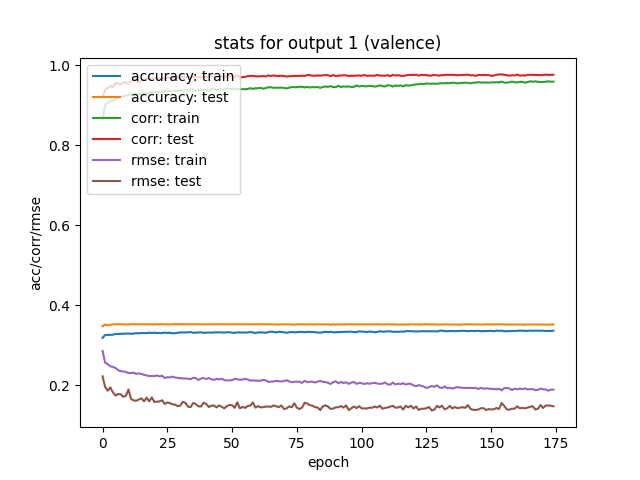
\includegraphics[angle=0, width=0.9\textwidth]{Figures/output1.png}
  \caption{Training progress for 'Valence'}
  \label{fig:TrainingProgressValence}
  \end{center}
\end{figure}

\begin{figure}[H]
  \begin{center}
  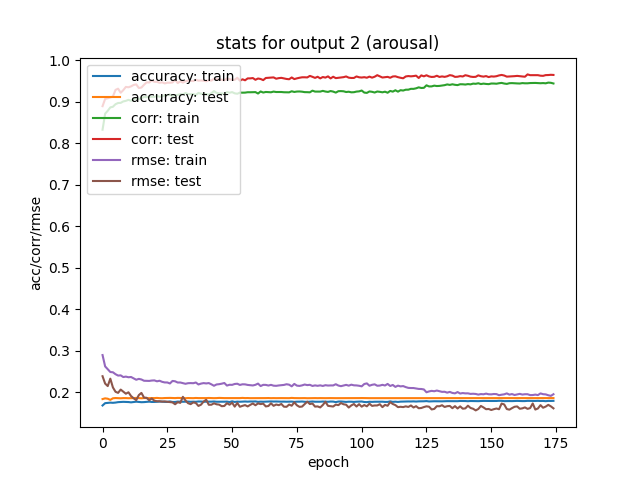
\includegraphics[angle=0, width=0.9\textwidth]{Figures/output2.png}
  \caption{Training progress for 'Arousal'}
  \label{fig:TrainingProgressArousal}
  \end{center}
\end{figure}

Even though these results are based on a 5-fold cross-validation, as done by two of the before mentioned papers, it is trained on completely shuffled data. Thus, training is not subject independent, which means, different frames from one specific person can appear in the training fold, as well as the testing fold. Implementing this, makes the training process harder and worse results are to be expected.
\newline\newline
The following table summarizes the results from a 5-fold cross-validation with subject-independent folds:
(Numbers can not be exactly specified, as they are being read from a chart)

\begin{table}[H]
\centering
\begin{tabular}{clll}
\multicolumn{1}{l}{\textbf{}} & \cellcolor[HTML]{9aff99}\textbf{ACC} & \cellcolor[HTML]{9aff99}\textbf{RMSE} & \cellcolor[HTML]{9aff99}\textbf{CORR} \\
\cellcolor[HTML]{F8FF00}\textbf{\begin{tabular}[c]{@{}c@{}}Valence\\ (out1)\end{tabular}} & 0.33 & 0.28 & 0.83 \\ \hline
\cellcolor[HTML]{F8FF00}\textbf{\begin{tabular}[c]{@{}c@{}}Arousal\\ (out2)\end{tabular}} & 0.18 & 0.26 & 0.80
\end{tabular}
\end{table}





\section{Results and comparison}
Comparing the above mentioned papers with the actual achieved results:

\begin{table}[H]
\begin{tabular}{clcc|cc}
\multicolumn{1}{l}{} & \multicolumn{1}{c}{\textbf{Architecture}} & \textbf{Evaluation} & \textbf{Metrics} & \multicolumn{1}{l}{\cellcolor[HTML]{9AFF99}\textbf{RMSE}} & \multicolumn{1}{l}{\cellcolor[HTML]{9AFF99}\textbf{CORR}} \\ \hline
\textbf{\begin{tabular}[c]{@{}c@{}}RESULTS\\ THESIS\end{tabular}} & \begin{tabular}[c]{@{}l@{}}CNN\\ (VGGFace)\end{tabular} & \begin{tabular}[c]{@{}c@{}}5-fold CV \end{tabular} & \cellcolor[HTML]{F8FF00}\textbf{\begin{tabular}[c]{@{}c@{}}average\\ V+A\end{tabular}} & 0.1288 & 0.9425 \\
\hline
\textbf{\begin{tabular}[c]{@{}c@{}}RESULTS\\ THESIS\end{tabular}} & \begin{tabular}[c]{@{}l@{}}CNN\\ (VGGFace)\end{tabular} & \begin{tabular}[c]{@{}c@{}}5-fold CV\\ subject indep.\end{tabular} & \cellcolor[HTML]{F8FF00}\textbf{\begin{tabular}[c]{@{}c@{}}average\\ V+A\end{tabular}} & 0.27 & 0.815 \\ 
\hline
\begin{tabular}[c]{@{}c@{}}Paper\\ AFEW-VA\end{tabular} & MKL & \begin{tabular}[c]{@{}c@{}}5-fold CV\\ subject indep.\end{tabular} & \cellcolor[HTML]{F8FF00}\textbf{\begin{tabular}[c]{@{}c@{}}average\\ V+A\end{tabular}} & 0.2434 & 0.423 \\
\hline
\begin{tabular}[c]{@{}c@{}}Paper\\ AFEW-VA\end{tabular} & FT-DCNN & \begin{tabular}[c]{@{}c@{}}5-fold CV\\ subject indep.\end{tabular} & \cellcolor[HTML]{F8FF00}\textbf{\begin{tabular}[c]{@{}c@{}}average\\ V+A\end{tabular}} & 0.38 & 0.285 \\
\hline
\begin{tabular}[c]{@{}c@{}}Paper\\ DeepDriver\end{tabular} & CNN + LSTM & \begin{tabular}[c]{@{}c@{}}3-fold CV + training\\ on 2 different DBs\end{tabular} & \cellcolor[HTML]{F8FF00}\textbf{\begin{tabular}[c]{@{}c@{}}average\\ V+A\end{tabular}} & 0.09 & 0.6325 \\
\hline
\begin{tabular}[c]{@{}c@{}}Paper\\ CrossDB\end{tabular} & CNN & \begin{tabular}[c]{@{}c@{}}5-fold CV\\  subject indep.\end{tabular} & \cellcolor[HTML]{F8FF00}\textbf{\begin{tabular}[c]{@{}c@{}}average\\ V+A\end{tabular}} & 0.25 & 0,34
\end{tabular}
\end{table}

\section{Experiments}
\subsection{Data Augmentation}
Basis is the 5-fold cross-validation approach with subject independent testing and validation data. In comparison to the results mentioned above, adding data augmentation couldn't show any improvement in performance.
\newline\newline
This data augmentation was applied:
-
\newline\newline
These are the results for the rmse metric for valance and arousal:

\subsection{Regularization}
- BatchNormalization layer proved to provide constantly significant better results.
- Despite a paper\cite{Pittaras:2017:FineTuningStrategiesComparison} arguing that generally the best approach for finetuning is to only add one Dense Layer with a high number of neurons to the original pretrained model, the obtained results weren't automatically performing better, mostly worse.
\newline\newline
Validation loss during training is lower than the training loss, which is very likely because of the reason that regularization was applied. This L2 regularization is only applied during training, but not validation/testing, which explains the significant difference between those values.
https://www.pyimagesearch.com/2019/10/14/why-is-my-validation-loss-lower-than-my-training-loss/

\subsection{Experiment 1: LSTM}
with non-shuffled data in order to capture the time-spatio changes in frames and enhance the performance of ER through the detection of those changes.

\subsection{Experiment 2: MTCNN (Multi-task Cascaded Convolutional Neural Network)}
- How often does MTCNN fail to detect faces??
Out of 30051 frames it only failed to detect a face in 961 faces, this presents 3.2 percent of all images.
\newline\newline
- What happens when not using MTCNN and directly feeding the original images into the VGGFace model for fine tuning.

\subsection{Experiment 3: AAM (Active Appearance Model)}




